\cleardoublepage
\chapter[Band structures of semiconductors and insulators]{Band structures of semiconductors\break and insulators\label{ch:band-structures}}
In this chapter we discuss the details of practical calculations, and the results obtained for a manifold of reference insulating materials. Thanks to the validity of Bloch's theorem, discussed in \cref{ch:koopmans-periodic}, it is possible to obtain electronic band structures -- within the primitive cell's BZ -- either from a supercell approach, by means of an unfolding method, or from the primitive cell implementation described in \cref{sec:koopmans-pbc}. The computational details of the calculations, including the description of the unfolding method and of the Koopmans workflow, are discussed in \cref{sec:calculations-koopmans}, while in \cref{sec:results-bands} we report the obtained results.

Part of the content of this chapter, as well as the reported results, have been published in Refs.~\cite{de_gennaro_blochs_2022,colonna_koopmans_2022}.

\clearpage
\section{Calculations with Koopmans functionals\label{sec:calculations-koopmans}}
Electronic-structure calculations using Koopmans spectral functionals are performed following two different approaches, based on the two strategies to compute the screening parameters discussed in \cref{sec:screening-parameters}: the first makes use of the finite energy differences strategy and relies on the SC method to model the system deprived of a particle, the second resorts to linear response theory and takes full advantage of the system's symmetries by exploiting the Wannier-like nature of the variational orbitals.

The former represents the original approach used to perform the first calculations in crystalline materials \cite{nguyen_koopmans-compliant_2018}, although, in that case, the quasiparticle energies were computed only at the $\Gamma$-point of the SC (no information about the $\bk$-dispersion). By means of an unfolding technique -- which, once again seizes on the fact that the variational orbitals are WFs, to reconstruct the $\bk$-dependence of the Koopmans Hamiltonian -- here we show, for the very first time, band structures calculations from Koopmans functionals along any path in the BZ \cite{de_gennaro_blochs_2022} (from now on, when speaking of the BZ, we will implicitly refer to the PC's BZ, since the one corresponding to the SC always consists of the $\Gamma$-point only).

The second approach came out more recently \cite{colonna_koopmans_2022} and relies on a second-order approximation of the $\Pi_i$ terms which, for the moment, has been developed only for the KI functional. On the bright side, the linear response approach does not require to compute the self-consistent energies of system with an additional electron or hole -- the screening parameters are computed directly on the neutral system via density-functional perturbation theory (DFPT) -- which makes the calculations much more simple and computationally feasible with respect to the SC approach. Although most of the work carried out in this thesis was performed using the SC approach, in this chapter we will describe also the PC implementation and show some results obtained with this method.

A big part of this thesis was dedicated to the development of some parts of the computational code, to reach a stable implementation working for periodic systems, together with an optimization of the entire workflow required to perform calculations of Koopmans functionals in crystalline materials. In the following sections we give a detailed description of these aspects.


\subsection{Unfolding and interpolation method\label{sec:unfolding-method}}
When simulating a bulk crystalline material, the infinite system is usually studied with Born-von Karman (BvK) boundary conditions, which introduce a discretization of the $\bk$-points inside the BZ. Equivalently, one can study explicitly the BvK supercell containing the $N$ periodic replicas of the primitive cell but, as was already mentioned, in this case one no longer has direct access to the band structure of the primitive cell.

\begin{figure}
    \centering
    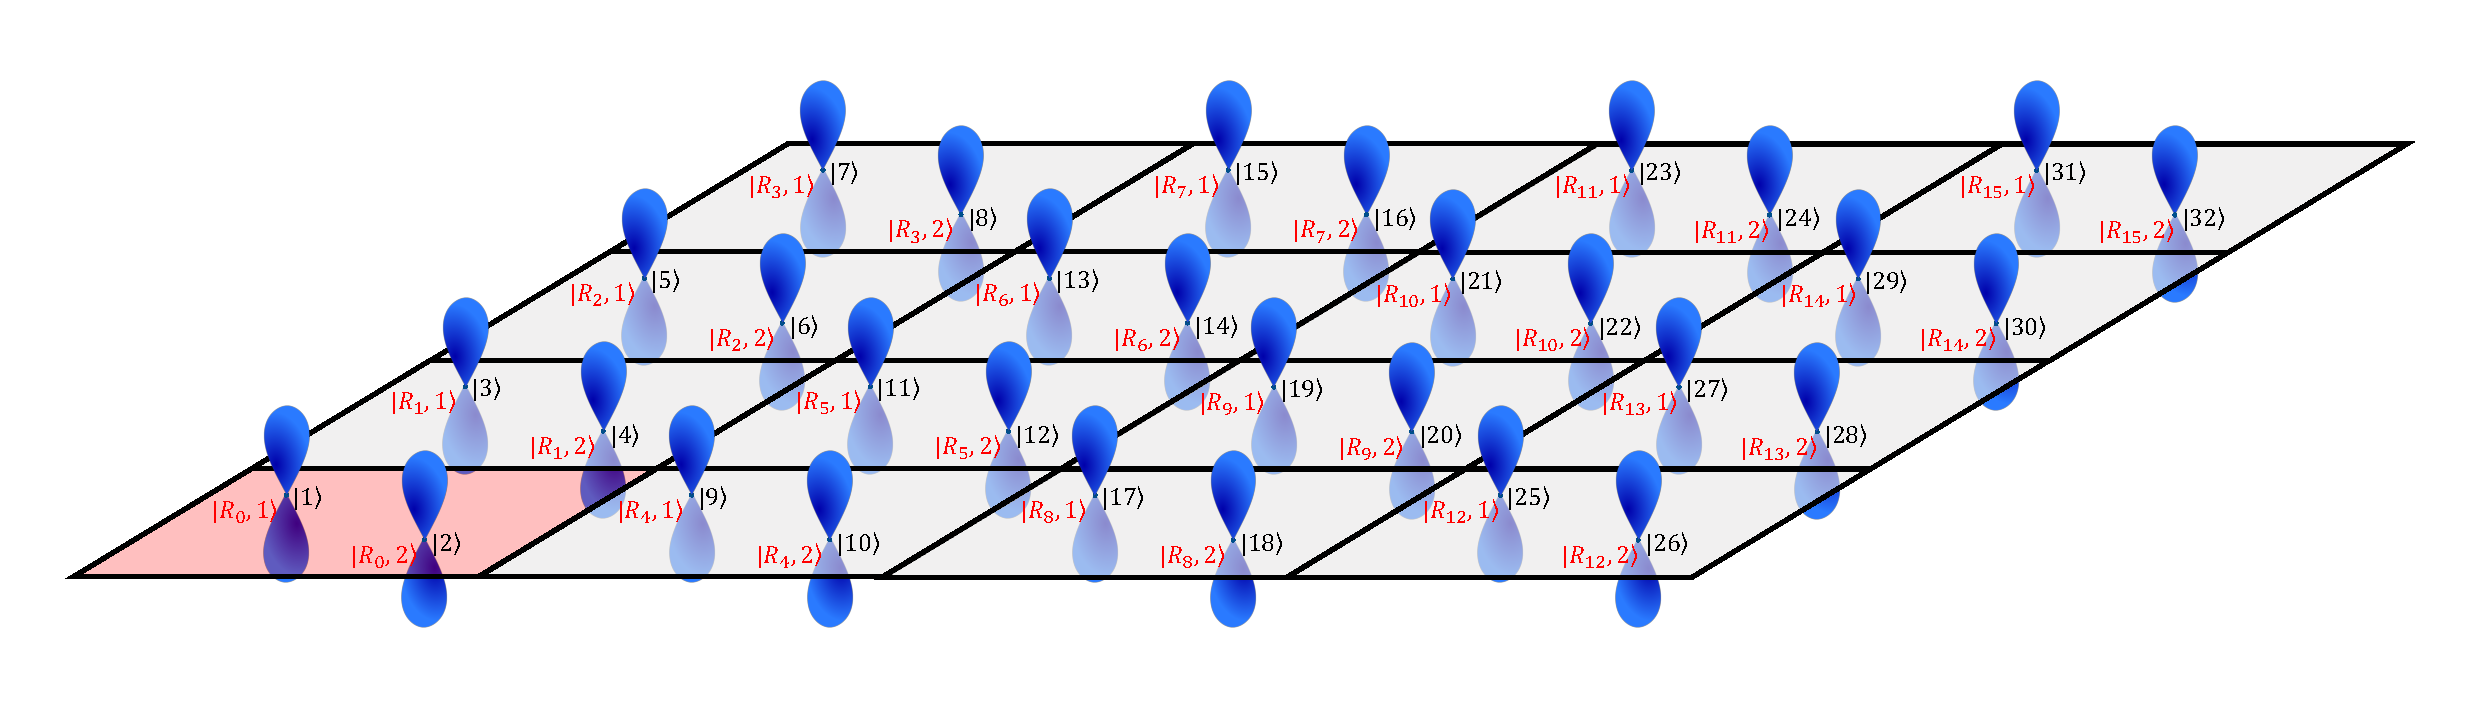
\includegraphics[width=\linewidth]{WF-pcell-scell.pdf}
    \caption[Schematic representation of the map connecting PC's and SC's Wannier functions]{Schematic representation of a two-dimensional 2-band model showing the connection between the PC and SC Wannier representations. In the primitive picture with a $4\times 4$ sampling of the BZ, the WFs are identified with the pair of labels $\{ n,\bR \}$ (red labels): the cell index $\bR$ taking four values and the band index $n$ taking two values. In the $4\times 4$ SC with $\Gamma$-sampling of the BZ, the eight WFs are labeled by only one quantum number (black labels), i.e.\ the SC band index $\alpha$ running over the eight states.}
    \label{fig:map-wf}
\end{figure}

In order to recover this band structure, several methods have been developed \cite{boykin_practical_2005, lee_band_2005, ku_unfolding_2010, popescu_extracting_2012, huang_general_2014, medeiros_effects_2014, zheng_quantum_2015}; our approach follows the same strategy of \cite{lee_band_2005} and exploits the Wannier nature of the variational orbitals. By means of the transformation linking WFs and BFs [see \cref{eq:wannier-function}], the matrix elements of the $\bk$-space Hamiltonian are obtained from those given by the Wannier-like variational orbitals via a (double) Fourier transform:
%
\begin{equation}
    \begin{split}
        h^{\rm KC}_{mn}(\bk,\bk') &= \sum_{\bR,\bR'} e^{-i\bk \cdot \bR} e^{i\bk' \cdot \bR'} \braket{w_{m\bR} | \hat{h}^{\rm KC}_{n\bR'} | w_{n\bR'}} \\
        &= \sum_{\bR,\bR'} e^{-i\bk \cdot \bR} e^{i\bk' \cdot \bR'} h^{\rm KC}_{mn}(\bR,\bR') ,
    \end{split}
    \label{eq:double-k-ham}
\end{equation}
%
where we introduced the matrix elements $h^{\rm KC}_{mn}(\bR,\bR') = \braket{w_{m\bR} | \hat{h}^{\rm KC}_{n\bR'} | w_{n\bR'}}$. If the Koopmans Hamiltonian is compliant with the translation symmetries of the system, the matrix elements satisfy the property
%
\begin{equation}
    \begin{split}
        h^{\rm KC}_{mn}(\bR,\bR') &= \braket{w_{m\bR} | \hat{h}^{\rm KC}_{n\bR'} | w_{n\bR'}} \\
        &= \braket{w_{m{\bm 0}} | \hat{h}^{\rm KC}_{n\bR'-\bR} | w_{n\bR'-\bR}} \\
        &= h^{\rm KC}_{mn}({\bm 0},\bR'-\bR) \equiv h^{\rm KC}_{mn}(\bR'-\bR) ,
    \end{split}
    \label{eq:trans-prop-koopmans-matrix-elements}
\end{equation}
%
that, if used in \cref{eq:double-k-ham}, yields a block-diagonal matrix (as expected from Bloch's theorem)
%
\begin{equation}
    h^{\rm KC}_{mn}(\bk,\bk') = h^{\rm KC}_{mn}(\bk) \delta(\bk - \bk')
    \label{eq:block-diagonal-koopmans-ham}
\end{equation}
%
with
%
\begin{equation}
    h^{\rm KC}_{mn}(\bk) = \sum_{\bR} e^{i \bk \cdot \bR} \braket{w_{m\bm{0}} | \hat{h}^{\rm KC}_{n\bR} | w_{n\bR}} = \sum_{\bR} e^{i \bk \cdot \bR} h^{\rm KC}_{mn}(\bR) ,
    \label{eq:hk-unfold}
\end{equation}
%
The diagonalization of the Hamiltonian with matrix elements defined by \cref{eq:hk-unfold}, yields the quasiparticle energies $\varepsilon_{n\bk}$ at any $\bk$-point.

In the SC approach the Brillouin zone reduces to a single point; as a consequence, the SC Hamiltonian in the Wannier representation loses the information about the lattice vectors $\{\bR\}$ and its matrix elements are labeled by the SC index only. In order to reconstruct the $\bk$-space Hamiltonian of \cref{eq:hk-unfold}, one must reconstruct the composite index $\{n,\bR\}$ of each WF from its supercell-picture index ${\alpha}$ (see \cref{fig:map-wf}). An effective way to do this is to first choose a reference PC and define the orbitals with the centers inside it as the ``$\bR=\bm{0}$ Wannier functions''. The second step consists of comparing all the other WFs in the supercell with those in the reference cell. If the Wannier translation property holds, we are able to connect each WF to its reference function $w_{\bm{0} n}$ and lattice vector $\bR$, defined as the distance between the centers of the two functions. If the system has more functions sharing the same center, one can look at the second-order moments ($\braket{x^2}$, $\braket{y^2}$, $\braket{z^2}$) to have a more detailed signature of WFs and, if needed, can move towards higher-order spatial moments until the character of each Wannier function is unequivocally defined \cite{shelley_automated_2011}.

As argued in Ref.~\cite{lee_band_2005}, \cref{eq:hk-unfold} not only applies to the points belonging to the $\bk$-mesh commensurate with the chosen supercell, but it is also an excellent interpolator. So, in order to calculate the band structure along any path in the Brillouin zone, we obtain the matrix elements of the $\bk$-space Hamiltonian by simply applying \cref{eq:hk-unfold} to any arbitrary $\bk$-point. In doing so, two approximations are applied to the matrix elements. To highlight such approximations -- and, especially, justify the fact that they have a negligible effect -- let us consider a point $\bk'$ which does not belong to the original sampling $\{ \bk \}$ of the BZ. In \cref{eq:hk-unfold}, the $\bk$-points must be commensurate\footnote{
A regular sampling of the BZ, made of $N_1 \times N_2 \times N_3$ $\bk$-points generates a system consisting of $N_1 \times N_2 \times N_3$ repetitions of the unit cell, each of which is identified by a lattice vector $\bR$; a set $\{ \bk \}$ which samples (regularly) the BZ is said to be commensurate to $\{ \bR \}$ (and viceversa) if the latter is the direct lattice with PBC set by $\{ \bk \}$.
}
with the set of lattice vectors $\{ \bR \}$ over which the sum runs, therefore, in order to compute the matrix elements $h^{\rm KC}_{mn}(\bk')$ we should, in principle, sum over a set $\{ \bR' \}$ which is commensurate to a sampling of the BZ that includes the point $\bk'$. When interpolating the matrix elements of the $\bk$-space Hamiltonian, we apply then a zero-padding technique \cite{buongiorno_nardelli_paoflow_2018}, where the contributions coming from the bigger lattice $\{ \bR' \}$ are neglected:
%
\begin{equation}
    \begin{split}
        h^{\rm KC}_{mn}(\bk') &= \sum_{\bR'} e^{i \bk' \cdot \bR'} \braket{w_{m\bm{0}} | \hat{h}^{\rm KC}_{n\bR'} | w_{n\bR'}}_{V'} \\
        &= \sum_{\bR} e^{i \bk \cdot \bR} \braket{w_{m\bm{0}} | \hat{h}^{\rm KC}_{n\bR} | w_{n\bR}}_{V'} + \sum_{\bR' \neq \bR} e^{i \bk \cdot \bR'} \braket{w_{m\bm{0}} | \hat{h}^{\rm KC}_{n\bR'} | w_{n\bR'}}_{V'} \\
        &\approx \sum_{\bR} e^{i \bk \cdot \bR} \braket{w_{m\bm{0}} | \hat{h}^{\rm KC}_{n\bR} | w_{n\bR}}_{V}
    \end{split}
    \label{eq:hk-interpolated}
\end{equation}
%
where $V$ and $V'$ are the volumes of the lattices $\{ \bR \}$ and $\{ \bR' \}$. In the last step the terms corresponding to lattice vectors not belonging to the original lattice -- i.e. $\bR' \neq \bR$ -- are neglected, and the integral to evaluate the matrix elements $h^{\rm KC}_{mn}(\bR)$ is calculated over the volume $V$ (rather than $V'$). The accuracy of the approximation is higher the smaller the contribution from these terms, i.e. the more localized the variational orbitals are, or the larger the supercell becomes. A poorly interpolated band structure is usually symptom of a significant contribution from the matrix elements corresponding to larger $\bR$-vectors, or of a non-negligible integral coming from the region $V' \setminus V$ in the calculation of the matrix elements $h^{\rm KC}_{mn}(\bR)$. Ultimately, the effects of such approximations are reduced by increasing the size of the supercell.

\subsubsection*{Smooth interpolation method}
As a consequence of what was just discussed, when reconstructing the band structure from a supercell calculation, one faces a trade-off: on one hand, a sufficiently large SC must be used to minimize the errors associated with neglecting long-range matrix elements of the Hamiltonian. But on the other hand, increasing the size of the SC dramatically increases the computational costs. In this scenario, one can exploit the fact that the Koopmans potential is a small, slowly varying correction on top of the original DFT Hamiltonian. If one decomposes the right-hand side of \cref{eq:hk-unfold} in its DFT and KC components,
%
\begin{equation}
    h^{\rm KC}_{mn}(\bR) \longrightarrow h^{\rm DFT}_{mn}(\bR) + v^{\rm KC}_{mn}(\bR) ,
\end{equation}
%
it is reasonable to assume that the major source of error comes from the interpolation of $h^{\rm DFT}_{mn}(\bR)$. This allows to improve the interpolation of the band structure by rewriting \cref{eq:hk-unfold} as
%
\begin{equation}
    h^{\rm KC}_{mn}(\bk) = \sum_{\bR'} e^{i \bk \cdot \bR'} h^{\rm DFT}_{mn}(\bR') + \sum_{\bR} e^{i \bk \cdot \bR} v^{\rm KC}_{mn}(\bR)
    \label{eq:hk-smooth}
\end{equation}
%
where the set of vectors $\{ \bR' \}$ now corresponds to a much larger supercell or, equivalently, it comes from a calculation with a denser $\bk$-points grid. This represents a significant saving in computational costs because the Koopmans calculation can be then performed on smaller supercells than would otherwise be necessary.

In order to have a consistent representation between (a) the DFT Hamiltonian defined  on a very dense grid, and (b) the KC potential on a coarser grid, it is important to have the same set of WFs for the two calculations. As long as this is fulfilled, the Koopmans Hamiltonian can be factorized as shown in \cref{eq:hk-smooth} and the DFT part can be obtained starting from a $\bk$-points grid dense enough to reliably interpolate the band structure.

We stress that this method has the one goal of improving the interpolation of the band structure. The convergence of other results, such as total energies and eigenvalues on the $\bk$-points grid commensurate with the supercell, is typically achieved with relatively small supercells. The technique depicted above does not affect any of these quantities and only improves the results for the electronic eigenvalues at $\bk$-points not included in the original Monkhorst-Pack grid.

\subsection{Workflow\label{sec:workflow}}
The full procedure to perform a full calculation of Koopmans functionals is rather complex, and follows different steps, each of which requires several calculations. 

\begin{figure}
    \centering
    \subfloat[]{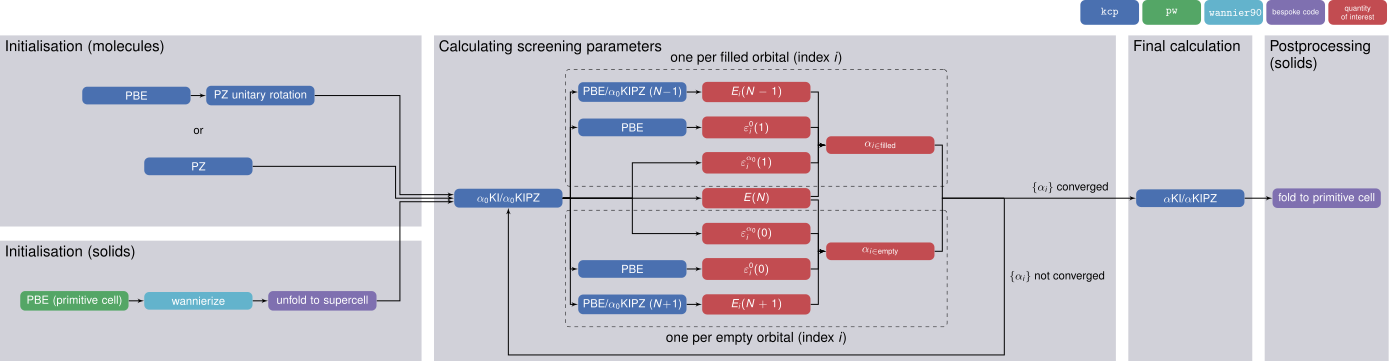
\includegraphics[width=\linewidth]{dscf_workflow.png}} \\
    \subfloat[]{
\includegraphics[width=\linewidth]{dfpt_workflow.png}}
    \caption[]{}
    \label{fig:workflow}
\end{figure}

\subsection{Computational details\label{sec:computational-details}}

\section{Results\label{sec:results-bands}}

\subsection{Finite differences\label{sec:results-dscf}}

\subsection{DFPT\label{sec:results-dfpt}}

